%This work is licensed under the Creative Commons
%Attribution-ShareAlike 4.0 International License. To view a copy of
%this license, visit http://creativecommons.org/licenses/by-sa/4.0/ or
%send a letter to Creative Commons, PO Box 1866, Mountain View, CA
%94042, USA.

%This work is licensed under the Creative Commons
%Attribution-ShareAlike 4.0 International License. To view a copy of
%this license, visit http://creativecommons.org/licenses/by-sa/4.0/ or
%send a letter to Creative Commons, PO Box 1866, Mountain View, CA
%94042, USA.

%\documentclass[gray,handout, pdftex, 11pt]{beamer}
%\documentclass[handout, pdftex, 11pt]{beamer}

\documentclass[pdftex, 11pt]{beamer}

\usepackage[utf8]{inputenc}
\usepackage[T1]{fontenc}
\usepackage{lmodern}
%\usepackage[italian]{babel}
\usepackage{graphicx}
\usepackage{listings}
\usepackage{microtype}
\usepackage{acronym}
\usepackage{array}
\usepackage{tikz}
\usetikzlibrary{shapes, chains, scopes, shadows, positioning, arrows,
  decorations.pathmorphing, calc}

\colorlet{c1}{green!20}
\colorlet{c2}{blue!10}
\colorlet{drawColor}{black!50}
\colorlet{commentColor}{green!70!black!90}

\tikzstyle{oval}=[ellipse, align=center, drop shadow, draw=drawColor, fill=white]
\tikzstyle{rect}=[rectangle, rounded corners=2pt, align=center, drop
shadow, draw=drawColor, fill=white]
\tikzstyle{comment}=[text=commentColor,font=\itshape]
\tikzstyle{textLab}=[]
\tikzstyle{arrow}=[->, very thick, >=stealth', draw=black!80]
\tikzstyle{darrow}=[->, dash pattern=on 3pt off2pt, very thick, >=stealth', draw=black!80]
\tikzstyle{fStartEnd}=[ellipse, align=center, drop shadow, draw=drawColor, fill=white]
\tikzstyle{fInput}=[trapezium, trapezium left angle=70, trapezium right angle=110,
align=center, drop shadow, draw=drawColor, fill=white]
\tikzstyle{fProcess}=[rectangle, align=center, drop shadow, draw=drawColor, fill=white]
\tikzstyle{fSelection}=[diamond, shape aspect=3, align=center, drop
shadow, draw=drawColor, fill=white]
\tikzstyle{fOutput}=[tape, tape bend top=none, align=center, drop shadow, draw=drawColor, fill=white]
\tikzstyle{mem}=[rectangle, align=center, draw=drawColor, fill=white]
\tikzstyle{clo}=[cloud, aspect=2, align=center, drop shadow, draw=drawColor, fill=white]

\lstdefinestyle{customc}{
   language=C,
   % basicstyle=\small\ttfamily\bfseries,
   basicstyle=\ttfamily,
   keywordstyle=\color{blue}\ttfamily,
   stringstyle=\color{red}\ttfamily,
   commentstyle=\color{green}\ttfamily,
   morecomment=[l][\color{magenta}]{\#},
   % breaklines=false,
    breaklines=true, breakatwhitespace=false,
   frameround=fttt,
   frame=trBL,
   backgroundcolor=\color{yellow!20},
   numbers=left,
   stepnumber=1,    
   firstnumber=1,
   numberfirstline=true,
   numberstyle=\tiny\color{black!50},
   xleftmargin=2em,
   framexleftmargin=1.5em
   % linewidth=8cm,
}

\lstnewenvironment{cblock}[1][]
{
  \lstset{
    style=customc,
    #1
  }
}{}

\newcommand{\cfile}[2][]{
  \lstinputlisting[style=customc, #1]{#2}
}

\definecolor{links}{HTML}{2A1B81}
\hypersetup{colorlinks,linkcolor=links,urlcolor=links}

\definecolor{links}{HTML}{2A1B81}
\hypersetup{colorlinks,linkcolor=,urlcolor=links}


\mode<presentation>{
  %-------------------------1
  \usetheme{Boadilla}
  \usecolortheme{beaver}
  %-------------------------1
  %-------------------------2
  %\usetheme{Goettingen}
  %\usecolortheme{sidebartab}
  %-------------------------2
  %\useoutertheme[right]{sidebar}
  %\usefonttheme{default}
  \setbeamercovered{transparent}
  %\setbeameroption{show notes on second screen=right}
  \setbeamertemplate{navigation symbols}{}
  \setbeamertemplate{footline}{}

  \bibliographystyle{abbrv}  
  %\renewcommand\bibfont{\scriptsize}
  \setbeamertemplate{bibliography item}{\textbullet}
  \setbeamertemplate{itemize item}{\checkmark}
  \setbeamertemplate{itemize subitem}{-}
  \setbeamertemplate{enumerate items}[default]
  \setbeamertemplate{sections/subsections in toc}[square]
}

\subtitle{Logical Computational Thinking}
\institute[Tecnológico de Monterrey]{
  
\includegraphics[width=5cm]{img/logoTEC.jpg}\\[5mm]
  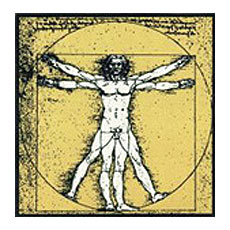
\includegraphics[width=1cm]{img/logoLEO.jpg}
  Scuola Leonardo Da Vinci (Firenze)
}

\author[Stefano Martina]{
  %\\[0.2cm]
  \textbf{Stefano MARTINA}\\
  {\small stefano.martina@gmail.com}
}

\titlegraphic{\tiny
  \href{http://creativecommons.org/licenses/by-sa/4.0/}{
\includegraphics[width=1cm]{img/logoCC.png}}
  This work is licensed under a
  \href{http://creativecommons.org/licenses/by-sa/4.0/}{Creative
    Commons Attribution-ShareAlike 4.0 International License}.}


\title[Lesson 4]{\textbf{Lesson 4 - Shell and \texttt{gcc} basics}}
\date[17/9/15]{\flushright 17 September 2015}

\begin{document}

\begin{frame}[plain]
  \titlepage
\end{frame}

\begin{frame}
  \frametitle{\bash\ shell}
  \begin{block}{What is a shell}
    Is a program that interprete commands given by the user. \C\
    programs can use the shell for basic input/output.
  \end{block}
  \begin{block}{important commands}
    \begin{itemize}
    \item \bb{pwd}: stands for Print Working Directory, print the
      current path, with directories separated by \bb{/}
    \item \bb{ls}: list the content of the current directory, you can
      add the option \bb{-l} for detailed output and \bb{-a} for
      seeing also hidden files
    \item \bb{cd path}: change the current directory to \bb{path}, can
      be also a \bb{nested/path} and \bb{cd /} go to the root, \bb{cd
        ~} or \bb{cd} go to the user's home (in Cygwin the home is not
      the windows home)
    \item \bb{./name}: for launching an executable called \bb{name}
      inside current path
    \end{itemize}
  \end{block}
\end{frame}

\begin{frame}
  \frametitle{\gcc\ (GNU C compiler)}
    \begin{block}{What is a compiler}
      Transform a source code in something executable from the
      machine.
    \end{block}
    \begin{center}
      \begin{tikzpicture}[node distance=17mm]
        \node (source)
        [file, label=above:\texttt{sName.c}, fill=c1]
        {\C\ source code};
        \node (obj)
        [file, label=above:\texttt{oName.o}, right=of source, fill=c2]
        {Object file};
        \node (libs)
        [files, label={[label distance=1mm]above:\texttt{libs.h}}, below=7mm of obj, fill=c3]
        {Libraries};
        \node (exe)
        [file, label=above:\texttt{eName\{.exe\}}, right=of obj, fill=c4]
        {Executable};
        \draw [arrow] (source) -- node [above, color=red] {compile} (obj);
        \draw [arrow] (obj) -- node [above, color=red] {link} (exe);
        \draw [arrow] (libs.east) -- ($ (exe.west) - (8mm,0) $);

      \end{tikzpicture}    
    \end{center}
    \begin{itemize}
    \item \alert{Compile:} \bb{gcc -c sName.c -o oName.o}; if \bb{-o}
      option not present, automatically use \bb{sName.o} as name
    \item \alert{Link:} \bb{gcc oName.o -o eName}; if \bb{-o}
      option not present, automatically use \bb{a.out} as name
    \item \underline{\alert{Compile + link:} \bb{gcc sName.c -o eName}}
    \end{itemize}
\end{frame}

\begin{frame}
  \frametitle{Steps for building a program}
  \begin{enumerate}
  \item Open a \alert{text editor}
  \item\label{point:write} \alert{Write} the code (or open and modify an existing one)
  \item\label{point:path} \alert{Save} the file in a known path and with the
    extension \bb{.c} (i.e. \bb{name.c})
  \item Open the \alert{shell} (Cygwin for Windows, Terminal for Mac)
  \item Go to the same \alert{path} of the point~\ref{point:path}; use
    \bb{cd} and remember that the path to \texttt{Documents} is:
    \begin{itemize}
    \item for Windows with Cygwin: \texttt{/cygdrive/c/Users/[YourName]/Documents}
    \item for Mac: \texttt{\~/Documents}
    \end{itemize}
  \item \alert{Compile} the program with \bb{gcc name.c -o name}
  \item \alert{Execute} the program with \bb{./name}
  \item If you are happy with the result finish, otherwise go to
    point~\ref{point:write} with the same file
  \end{enumerate}
\end{frame}
\end{document}
